\section{Methodology: Video Comprehension Score (VCS)} % From template

\label{sec:methodology_vcs} % Add a label for the main section if you like

Figure~\ref{fig:VCS} illustrates the overall architecture of the Video Comprehension Score (VCS), a metric designed for the comprehensive evaluation of dense, long-form video descriptions. VCS assesses the quality of model-generated text ($\Tgen$) against a reference text ($\Tref$) by quantifying both semantic and narrative alignment. This approach aims to surpass traditional n-gram-based metrics by specifically addressing challenges such as the "many-to-one mapping" problem and the critical aspect of event ordering for narrative coherence. The subsequent subsections detail the fundamental components, preprocessing techniques, and the suite of metrics that constitute the VCS.

\subsection{Fundamental Components and Preprocessing} % From template
\label{sec:fundamental_components_revised} % From new text
\subsubsection{Core Technologies: Segmentation and Embedding} % From template
\label{ssec:core_technologies_revised} % From new text
VCS employs two core technologies. \SaT\ \cite{frohmann2024segment} segments texts into granular semantic segments for robust comparison of potentially noisy inputs. Subsequently, $\nvEmbed$\cite{lee2024nv} converts textual units (full texts and chunks) into high-dimensional vector embeddings, enabling quantitative similarity measurement.

\subsubsection{Text Preprocessing: Segmentation and Chunking for VCS} % Title from new text (more specific)
\label{sssec:text_preprocessing_and_chunking_revised} % From new text
For standard VCS (long-form descriptions), input texts $\Tref$ and $\Tgen$ are cleaned, typically involving removal of punctuation and full stops. \SaT\ \cite{frohmann2024segment} then segments these into sequences of semantic segments, $\Sref$ and $\Sgen$. To balance granularity and context, $k$ consecutive segments form "chunks," resulting in sequences $\Cref$ and $\Cgen$. These chunks are embedded using $\nvEmbed$\cite{lee2024nv} into matrix representations $\ECref \in \mathbb{R}^{\Nref \times D}$ and $\ECgen \in \mathbb{R}^{\Ngen \times D}$, crucial for LAS and NAS.

\subsection{VCS Metric Suite} % From template
\label{sec:vcs_metric_suite_revised} % From new text
The following components (GAS, LAS, NAS) and aggregation methods form the basis of VCS and $\VCSshort$.
\subsubsection{Global Alignment Score (GAS)} % From template
\label{ssec:gas_revised} % From new text
GAS measures overall semantic similarity between $\Tref$ and $\Tgen$. Entire texts $\Tref$ and $\Tgen$ are embedded via $\EmbedNVTwo$\cite{lee2024nv} to yield $\Erefvec$ and $\Egenvec$, respectively. GAS is their cosine similarity:
\begin{equation} \label{eq:gas_revised}
\text{GAS} = \cos(\Erefvec, \Egenvec) = \frac{\Erefvec \cdot \Egenvec}{\|\Erefvec\| \|\Egenvec\|}
\end{equation}
GAS captures thematic congruence but overlooks local agreement and chronology, addressed by LAS (Section~\ref{ssec:las_revised}) and NAS (Section~\ref{ssec:nas_revised}).

\subsubsection{Establishing Chunk Correspondences} % From template
\label{ssec:chunk_correspondences_revised} % From new text
To enable fine-grained comparison, VCS establishes one-to-one correspondences between text chunks (or words for $\VCSshort$).

\paragraph{Mapping Window Calculation} % Title from new text (no period)
\label{sssec:mapping_window_revised} % From new text
Mapping Windows (MW) define permissible alignment ranges for chunks/words between $\Tref$ and $\Tgen$, accommodating length and detail variations. Based on element counts $\Nref, \Ngen$ (chunks or words), their ratio $r = \max(\Nref, \Ngen) / \min(\Nref, \Ngen)$, and a base window height $h_{mw} = \lceil r \rceil$, VCS defines Precision Windows ($\MWprec$) for matching $\cjgen$ to $\ciref$, and Recall Windows ($\MWrec$) for matching $\ciref$ to $\cjgen$. These windows constrain the Best Matching Algorithm. Figure~\ref{fig:mapping_windows} illustrates MWs for cases of equal length, concise generation, and verbose generation.
\begin{figure}[ht] % You can adjust placement options like [htbp]
  \centering
  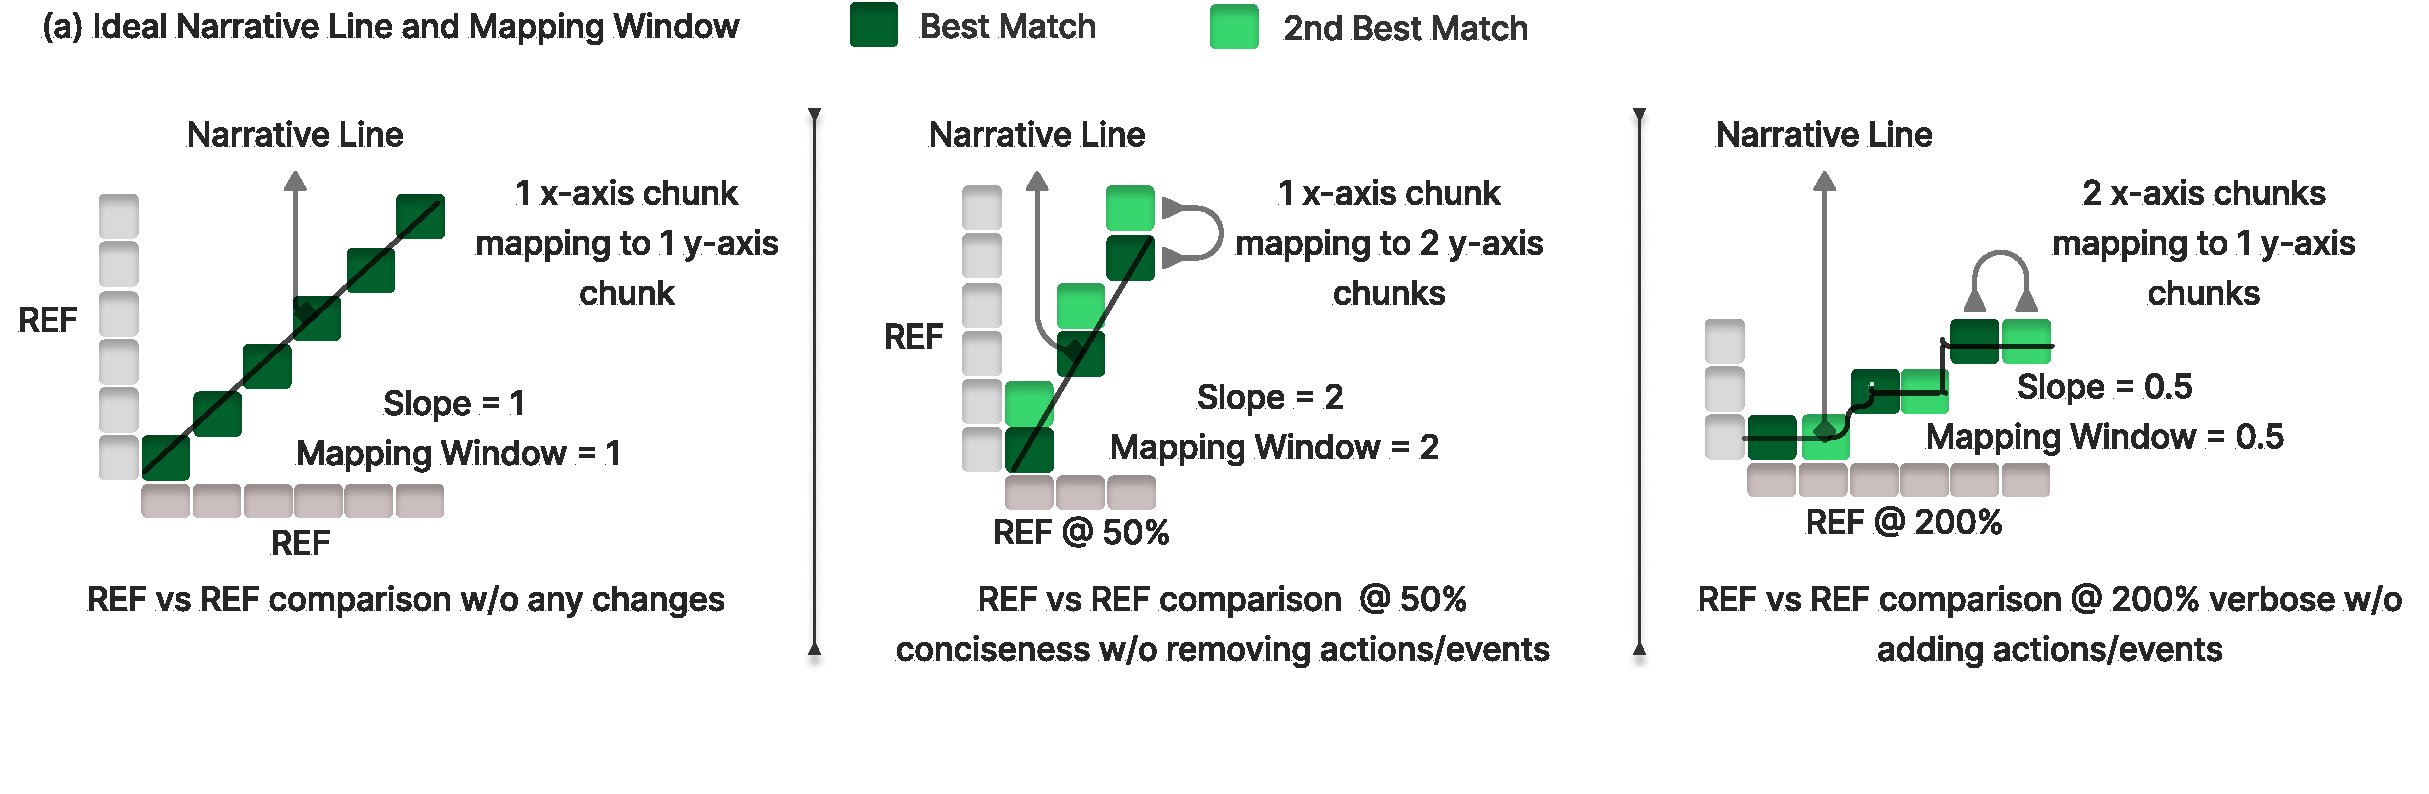
\includegraphics[width=1\textwidth]{mapping_window.pdf} % Adjust width as needed, or use other options like scale, height.
  \caption{Illustration of Mapping Windows: (a) Ideal 1-to-1, (b) Concise $\Tgen$ (e.g., 1 ref chunk to 2 gen chunks), (c) Verbose $\Tgen$ (e.g., 2 ref chunks to 1 gen chunk).}
  \label{fig:mapping_windows} % Optional: for cross-referencing the figure in your text
\end{figure}

\paragraph{Best Matching Algorithm} % Title from new text (no period)
\label{sssec:best_matching_revised} % From new text
The Best Matching Algorithm establishes robust one-to-one chunk/word correspondences, resolving semantic ambiguity and collisions inherent in naive highest-similarity pairing. For each source element, it identifies the maximum similarity ($\Mj$). If $\Mj$ exceeds a context cutoff (e.g., 0.6), an adaptive similarity margin (influenced by $\Mj$) defines a candidate band. From candidates within this band, the one closest to its expected narrative position (defined by $\MWprec$ or $\MWrec$) is selected. Ties are broken by highest raw similarity. This bidirectional process yields precision-oriented ($\MP$) and recall-oriented ($\MR$) best matches.

\subsubsection{Local Alignment Score (LAS)} % From template
\label{ssec:las_revised} % From new text
The Local Alignment Score (LAS) assesses fine-grained semantic quality, averaging cosine similarities of matched chunk/word pairs from Section~\ref{sssec:best_matching_revised}. It computes precision-oriented $\LASP = \frac{\sum_{(c_{j}^{\text{gen}},c_{m(j)}^{\text{ref}})\in \MP}\Sim(c_{j}^{\text{gen}},c_{m(j)}^{\text{ref}})}{|\MP|}$ (if $|\MP|>0$, else 0) and recall-oriented $\LASR = \frac{\sum_{(c_{i}^{\text{ref}},c_{m(i)}^{\text{gen}})\in \MR}\Sim(c_{i}^{\text{ref}},c_{m(i)}^{\text{gen}})}{|\MR|}$ (if $|\MR|>0$, else 0). The final LAS is their harmonic mean:
\begin{equation} \label{eq:las_revised}
\LAS = F_1(\LASP, \LASR) =
\begin{cases}
\frac{2 \cdot \LASP \cdot \LASR}{\LASP + \LASR} & \text{if } \LASP + \LASR > 0 \\
0 & \text{otherwise}
\end{cases}
\end{equation}
High LAS indicates strong local semantic agreement. LAS is somewhat sensitive to content gaps, though less so than NAS, and is insensitive to chronological order, motivating the Narrative Alignment Score (NAS) (Section~\ref{ssec:nas_revised}).

\subsubsection{Narrative Alignment Score (NAS)} % From template
\label{ssec:nas_revised} % From new text
The Narrative Alignment Score (NAS) evaluates narrative integrity and chronological coherence of $\Tgen$ against $\Tref$, addressing LAS's insensitivity to order and providing stronger penalties for structural discrepancies. For $\VCSshort$, NAS assesses word order.

\paragraph{Distance-based NAS ($\NASD$)} % Title from new text (no period)
\label{sssec:nasd_revised} % From new text
$\NASD$ assesses chronological alignment by penalizing deviations of matched elements ($\MP, \MR$) from expected positions within Mapping Windows (Section~\ref{sssec:mapping_window_revised}). It is largely sensitive to global misalignments (penalized more) and somewhat to local misalignments and content gaps. For each match, an effective distance $\dprime$ (incorporating LCT, Section~\ref{sssec:lct_revised}) contributes to a total penalty $\Ptotalx$. Normalizing by maximum possible penalty $\Pmaxx$ (Fig.~\ref{fig:max_penalty}) yields $\NASDP$ and $\NASDR$:
\begin{figure}[ht] % You can adjust placement options like [htbp]
  \centering
  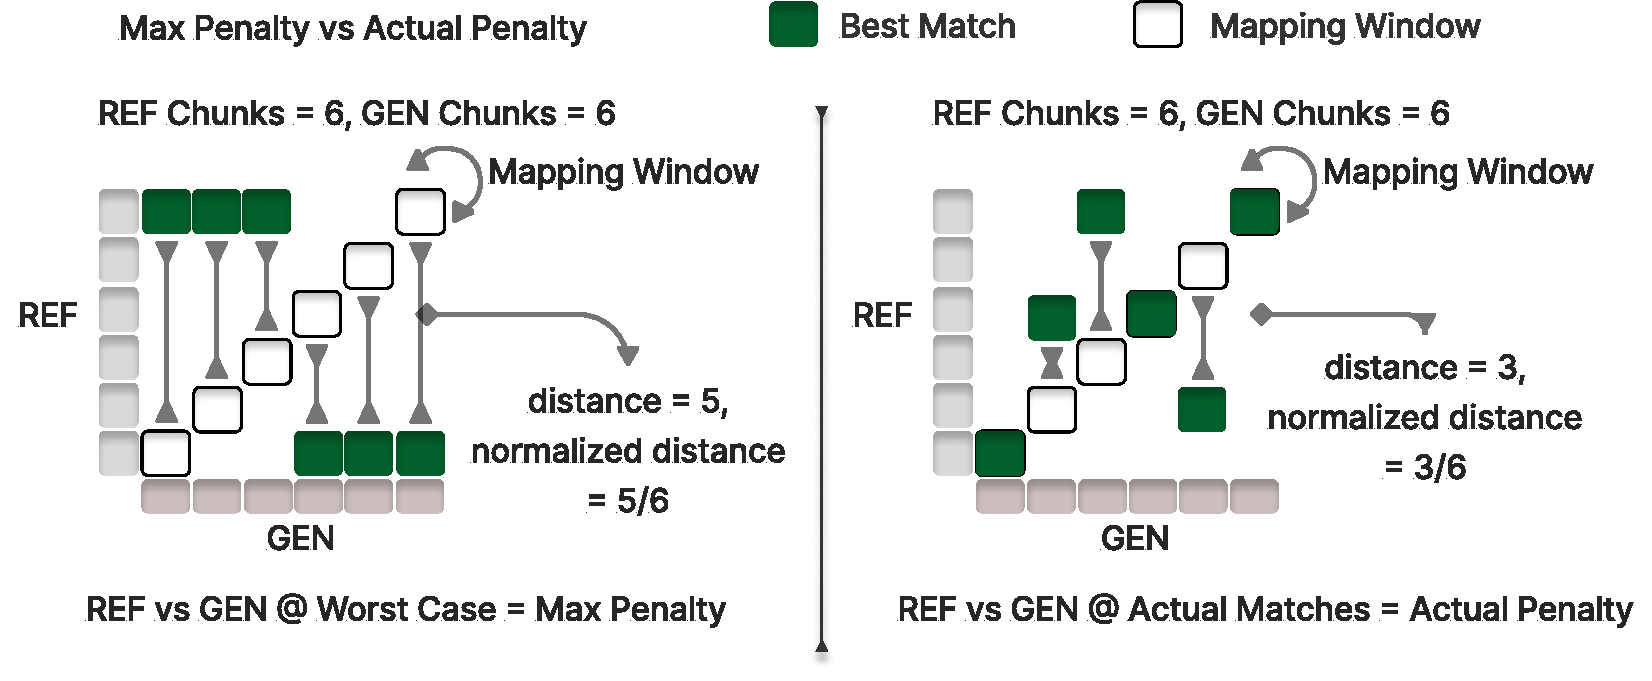
\includegraphics[width=1\textwidth]{MaxP.pdf} % Adjust width as needed, or use other options like scale, height.
  \caption{Illustration of Mapping Windows: (a) Ideal 1-to-1, (b) Concise $\Tgen$ (e.g., 1 ref chunk to 2 gen chunks), (c) Verbose $\Tgen$ (e.g., 2 ref chunks to 1 gen chunk).}
  \label{fig:max_penalty} % Optional: for cross-referencing the figure in your text
\end{figure}
\begin{equation} \label{eq:nas_dx_revised}
\text{NAS}_{Dx} =
\begin{cases}
1 - \frac{\Ptotalx}{\Pmaxx} & \text{if } \Pmaxx > 0 \\
1.0 & \text{if } \Pmaxx = 0 \text{ and } \Ptotalx = 0 \\
0.0 & \text{if } \Pmaxx = 0 \text{ and } \Ptotalx > 0
\end{cases}
\quad (x \in \{P, R\})
\end{equation}
$\NASD$ is the harmonic mean of $\NASDP$ and $\NASDR$:
\begin{equation} \label{eq:nas_d_revised}
\NASD = F_1(\NASDP, \NASDR)
\end{equation}

\paragraph{Line-based NAS ($\NASL$)} % Title from new text (no period)
\label{sssec:nasl_revised} % From new text
$\NASL$ evaluates local chronological flow by analyzing the path of consecutive matched elements. It is highly sensitive to local chronology and content gaps, and less sensitive to global misalignments compared to $\NASD$. An ideal path lies within an "ideal narrative band" (Fig.~\ref{fig:max_penalty}), bounded by estimated shortest ($\Lflooridealx$) and estimated longest ($\Lceilidealx$) path lengths. The actual path length ($\Lactualx$), from valid segment lengths (using LCT, Section~\ref{sssec:lct_revised}), is penalized for deviations:

\begin{equation} \label{eq:nas_lx_revised}
\text{NAS}_{Lx} =
\begin{cases}
1.0 & \text{if } \Lflooridealx \leq \Lactualx \leq \Lceilidealx \\
\Lactualx / \Lflooridealx & \text{if } \Lactualx < \Lflooridealx \text{ and } \Lflooridealx > 0 \\
\Lceilidealx / \Lactualx & \text{if } \Lactualx > \Lceilidealx \text{ and } \Lactualx > 0 \\
0.0 & \text{otherwise}
\end{cases}
\quad (x \in \{P, R\})
\end{equation}
$\NASL$ is the harmonic mean of $\NASLP$ and $\NASLR$:
\begin{equation} \label{eq:nas_l_revised}
\NASL = F_1(\NASLP, \NASLR)
\end{equation}

\paragraph{Local Chronology Tolerance (LCT)} % Title from new text (no period)
\label{sssec:lct_revised} % From new text
LCT (multiplier $\tauLCT \geq 0$) allows configurable flexibility for benign local reorderings and can add tolerance to minor content additions/omissions. In $\NASD$, it widens permissible deviation from Mapping Windows before penalty. In $\NASL$, it expands acceptable step variations between matches. $\tauLCT=0$ enforces strict order.

\paragraph{Final Narrative Alignment Score ($\NASFone$)} % Title from new text (no period)
\label{sssec:nas_f1_revised} % From new text
$\NASD$ (Eq.~\ref{eq:nas_d_revised}) and $\NASL$ (Eq.~\ref{eq:nas_l_revised}) are integrated via harmonic mean to produce $\NASFone$:
\begin{equation} \label{eq:nas_f1_revised}
\NASFone = F_1(\NASD, \NASL) 
\end{equation}

\paragraph{Window Regularizer for NAS} % Title from new text (no period)
\label{sssec:window_regularizer_revised} % From new text
The Window Regularizer ($\RW$) adjusts $\NASFone$ to mitigate influence from extreme text length disparities.
Let $MW_{\text{sel}}$ be $\MWrec$ if $\Nref < \Ngen$, else $MW_{\text{sel}} = \MWprec$.
Let $N_{\text{max}} = \max(\Nref, \Ngen)$.
The total mapping window area is $\Atotalmw = \sum_{(s,e) \in MW_{\text{sel}}} (e-s)$.
The timeline area is $\Atimeline = \Nref \cdot \Ngen$.
The minimum area ratio is $\Aminratio = 1/N_{\text{max}}$ (if $N_{\text{max}}>0$, else 0).
The Window Regularizer $\RW$ is calculated as:
\begin{equation}
\RW = 
\begin{cases}
\max\left(0, \min\left(1, \frac{(\Atotalmw / \Atimeline) - \Aminratio}{0.5 - \Aminratio}\right)\right) & \text{if } \Atimeline > 0 \text{ and } \Aminratio < 1 \\
0 & \text{otherwise}
\end{cases}
\end{equation}
The denominator term $(0.5 - \Aminratio)$ uses $0.5$ as a threshold because if the mapping windows cover 50\% or more of the total timeline area, the NAS score becomes significantly less meaningful due to overly relaxed chronological constraints, warranting the regularizer to approach its maximum effect.
Let $\NASinterim = \NASFone - \RW$. The regularized score $\NASreg$ is:
\begin{equation} \label{eq:nas_reg_revised}
\NASreg =
\begin{cases}
\frac{\NASinterim}{1 - \RW} & \text{if } \NASinterim > 0 \text{ and } \RW < 1 \\
0.0 & \text{otherwise}
\end{cases}
\end{equation}
This re-normalizes so $\NASreg$ can reach 1 if $\NASFone=1$ and $\RW=0$.

\subsection{Aggregating Scores for the Final Video Comprehension Score (VCS)} % From template
\label{sec:aggregating_scores_revised} % From new text
The final VCS or $\VCSshort$ integrates semantic and narrative alignment. GAS is modulated by LAS yielding the Semantic Alignment Score ($\SAS$):
\begin{equation} \label{eq:sas_revised} 
\SAS = 
\begin{cases}
\frac{\text{GAS} - (1 - \text{LAS})}{\text{LAS}} & \text{if } \text{LAS} > 0 \text{ and } (\text{GAS} - (1 - \text{LAS})) > 0 \\
0.0 & \text{otherwise}
\end{cases}
\end{equation}
The score (VCS or $\VCSshort$) synthesizes $\SAS$ with $\NASreg$ (Eq.~\ref{eq:nas_reg_revised}).
Let $S_{\text{num}}$ and $S_{\text{den}}$ be defined based on $\SAS$ and $\NASreg$:
\begin{align*}
S_{\text{num}} &= 
\begin{cases}
\SAS - (1 - \NASreg) & \text{if } \SAS < \NASreg \\
\NASreg - (1 - \SAS) & \text{otherwise}
\end{cases} \\
S_{\text{den}} &= 
\begin{cases}
\NASreg & \text{if } \SAS < \NASreg \\
\SAS & \text{otherwise}
\end{cases}
\end{align*}
The final score is:
\begin{equation} \label{eq:vcs_revised}
\text{VCS (or } \VCSshort\text{)} =
\begin{cases}
\frac{S_{\text{num}}}{S_{\text{den}}} & \text{if } S_{\text{num}} > 0 \text{ and } S_{\text{den}} \neq 0 \\
0.0 & \text{otherwise}
\end{cases}
\end{equation}

\subsection{\texorpdfstring{$\VCSshort$}{VCSshort}: Extension for Short Captions} % New section from new text
\label{sec:vcs_short} % From new text
VCS can be adapted for evaluating short captions at the word level, termed $\VCSshort$. The core metric suite (GAS, LAS, NAS) and aggregation logic (Section~\ref{sec:vcs_metric_suite_revised} and \ref{sec:aggregating_scores_revised}) remain consistent. The primary distinction lies in the initial text preprocessing.

\subsubsection{Text Preprocessing for \texorpdfstring{$\VCSshort$}{VCSshort}} % New subsection from new text
For $\VCSshort$, input texts $\Tref$ and $\Tgen$ are first cleaned by removing all punctuation and stop words. After this cleaning, the texts are tokenized into individual words. These words then serve as the fundamental "segments" or "elements" for all subsequent alignment and scoring processes, replacing the multi-word chunks used in the standard VCS. Each word is then embedded using $\nvEmbed$\cite{lee2024nv} for comparison. 